\subsubsection{Prophet} \label{sec:design-prophet}

OlaVM employs a reduced instruction set, which limits its ability to support certain complex computations. The conventional approach to address this is to implement such computations using existing instructions. 
However, this method may consume a large number of opcodes, and there is an upper limit on the size of Trace. 
Therefore, to accommodate more computations in Trace, each opcode should occupy fewer trace cells. Alternatively, one can take inspiration from the design of EVM and use a pre-compiled contract to support complex computations. 
In this mode, there is no need to use EVM instructions to implement the computation; instead, one can add the corresponding pre-compiled contract, which can be written in any high-level language such as Rust or Go. 
However, this approach significantly increases the proof workload, requiring a separate trace table for the complex computation, and performing constraint proof only on the output of this computation and its input recorded in the CPU trace.

\begin{figure}[!ht]
    \centering
    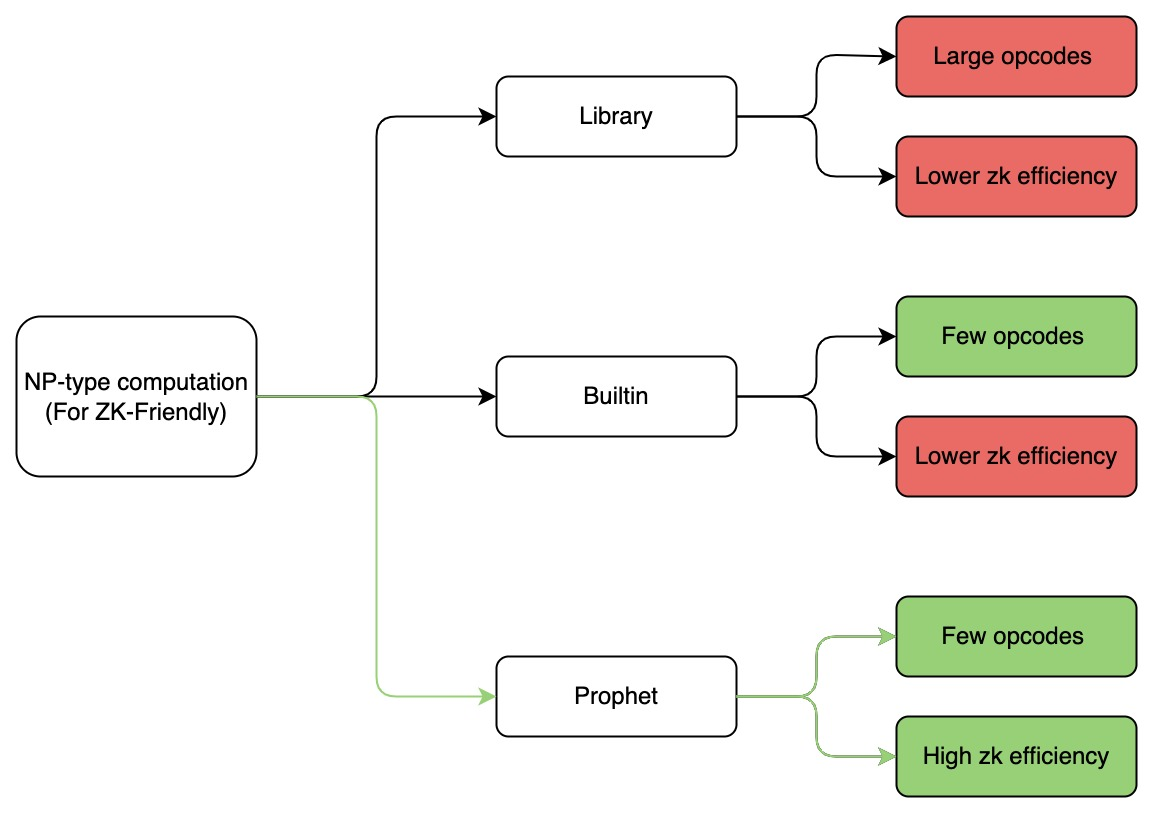
\includegraphics[width=0.5\textwidth]{vm/design-prophet.jpeg}
    \caption{How the Prophet can get ZK-Friendly}
    \label{fig:design-prophet}
\end{figure}

It is desirable to support complex computations using few opcodes without increasing the complexity of the proof. 
To achieve this, we have devised a method called the 'Prophet', depicted in \figref{fig:design-prophet}, 
which follows a prophecy and confirmation approach. This method fits well with the overall design of OlaVM.

For complex computations, the result of the complex computation is first computed locally by someone else (often Prover himself), without any constraints. 
Subsequently, the VM performs a validity check on the computed result before proceeding with the rest of the computation. 
This verification process is implemented using instructions and is included in the proof process.

For example, consider the task of calculating the square root of a radicand. 
While implementing Newton's method requires more than 20 instructions, verifying if a result is indeed the square root of a radicand can be done succinctly.
ZKVM, for instance, only needs to multiply the result with itself to obtain a product and then verify if the product is equal to the radicand. This process requires only two instructions. 
With the second algorithm, how to compute the square root is not a concern for the ZK circuit and user. The computation process is wrapped up in the prophet segment and does not need to be verified by the ZK circuit.
The ZK circuit only needs to verify the succinct logic $\texttt{result} \cdot \texttt{result} = \texttt{radicand}$. 
By using OlaVM to execute both algorithms and generate ZK proof, the second algorithm is ten times faster than the first traditional algorithm. (See Section \ref{subsec:prophet-interpreter} for more details.)

To ensure that OlaVM remains developer-friendly at a language level, it currently does not support developers to write their own Prophet implementations. 
Instead, the Prophet library is officially maintained and updated. Additionally, to ensure security, memory access during Prophet execution is read-only.
It's worth noting that not all complex calculations are suitable for this model. Calculations that are complex to implement but efficient to verify, such as square root and cube root, 
are more suitable for this approach. However, there are also some calculations that are not complex but still ZK-unfriendly, such as bitwise operations, range checks, hashing, and other calculations. 
These types of calculations are not suitable for Prophet's design. Instead, we use the pre-compiled approach to support them, which is similar to the pre-compiled contract function in EVM. 
We call this approach "Builtin". In the subsequent chapters, we will introduce the type of Builtin and the way of constraint in detail.